\documentclass[conference]{IEEEtran}

\usepackage{cite}
\usepackage{amsmath,amssymb,amsfonts}
\usepackage{algorithmic}
\usepackage{algorithm}
\usepackage{graphicx}
\usepackage{textcomp}
\usepackage{xcolor}
\usepackage{listings}
\usepackage{booktabs}
\usepackage{multirow}
\usepackage{url}
\usepackage{hyperref}
\usepackage{tikz}
\usetikzlibrary{arrows.meta,positioning,calc,fit,shapes.geometric,backgrounds}
\usepackage{etoolbox}
% Ensure algorithm text is always black (not white-on-white)
\AtBeginEnvironment{algorithmic}{\color{black}}

\lstset{
  basicstyle=\ttfamily\scriptsize,
  breaklines=true,
  frame=single,
  numbers=none
}

\def\BibTeX{{\rm B\kern-.05em{\sc i\kern-.025em b}\kern-.08em
    T\kern-.1667em\lower.7ex\hbox{E}\kern-.125emX}}

\begin{document}

\title{UpsideFuzzer: Coverage-Guided REST API Fuzzing for .NET\\
via Semantic Source-Aware Grammar Enhancement}

\author{\IEEEauthorblockN{Sergei Ovchinnikov}
\IEEEauthorblockA{sergey.o.a@gmail.com}
}

\maketitle

% ============================================================
\begin{abstract}
% ============================================================
We present \textbf{UpsideFuzzer}, an open-source greybox fuzzing framework for .NET REST APIs. The tool automatically extracts validation rules from C\# source code, enriches fuzz dictionaries with precise boundary values, instruments target binaries for edge coverage via SharpFuzz, and runs a coverage-guided fuzzing loop that sends structurally valid HTTP requests while using code-coverage feedback to decide what to explore next. In our evaluation, UpsideFuzzer discovered $127\%$--$169\%$ more unique code paths and up to $7\times$ more server crashes than the RESTler black-box baseline over a 24-hour campaign. A reproducible 20-minute benchmark on four public .NET services confirmed higher throughput and broader endpoint coverage. We also report results on five internal enterprise microservices, demonstrating the tool's practical applicability to production-grade .NET systems.
\end{abstract}

\begin{IEEEkeywords}
API fuzzing, coverage-guided fuzzing, greybox fuzzing, static analysis, .NET, REST API, instrumentation, OpenAPI
\end{IEEEkeywords}

% ============================================================
\section{Introduction: The Task and Its Relevance}
\label{sec:intro}
% ============================================================

REST APIs are the primary interface for most modern web services, mobile backends, and microservice architectures. Every public-facing endpoint is a potential entry point for an attacker. Finding bugs in these APIs before they reach production is one of the most important tasks in application security.

\textbf{Fuzzing} --- the practice of sending malformed or unexpected inputs to a program to provoke crashes and errors --- is a proven technique for finding bugs in binary programs. However, applying fuzzing to REST APIs is significantly harder than fuzzing a command-line tool or a file parser. The reason is straightforward: a REST API request must be valid at three levels simultaneously:

\begin{enumerate}
    \item \textbf{HTTP level:} the request must have a correct method, path, and headers.
    \item \textbf{JSON/body level:} the request body must be well-formed JSON (or XML, form-data, etc.).
    \item \textbf{Business-logic level:} the values in the body must pass the application's own validation rules --- string lengths, numeric ranges, enums, regex patterns, required fields, and more.
\end{enumerate}

If any of these layers rejects the input, the request is discarded before it reaches the deeper code where bugs actually live. The core challenge of API fuzzing is generating inputs that pass all three layers and reach the interesting logic.

\textbf{Our contribution.} UpsideFuzzer is a practical tool that combines three ideas into one pipeline: (1) grammar-based request generation from OpenAPI specifications, (2) automatic extraction of validation rules from C\# source code to generate better test values, and (3) coverage-guided feedback to steer the search toward unexplored code. This paper describes the full system, explains how each part works, and presents comparative evaluation results against the RESTler~\cite{restler_icse19} baseline.

% ============================================================
\section{Problem Statement: Why Existing Tools Fall Short}
\label{sec:problem}
% ============================================================

Before describing our solution, it is useful to understand why existing approaches are insufficient for thorough .NET API fuzzing. Table~\ref{tab:approach_comparison} summarizes the trade-offs.

\begin{table}[htbp]
\caption{Comparison of API Fuzzing Approaches}
\label{tab:approach_comparison}
\centering
\footnotesize
\resizebox{\columnwidth}{!}{%
\begin{tabular}{p{2.2cm}cccc}
\toprule
\textbf{Capability} & \textbf{Black-box} & \textbf{Coverage-} & \textbf{Upside-} \\
                     & \textbf{(RESTler)} & \textbf{guided (AFL)} & \textbf{Fuzzer} \\
\midrule
Valid HTTP structure   & \checkmark & $\times$ & \checkmark \\
Valid JSON bodies      & \checkmark & $\times$ & \checkmark \\
Stateful sequences    & \checkmark & $\times$ & \checkmark \\
Code coverage feedback & $\times$ & \checkmark & \checkmark \\
Source-aware values    & $\times$ & $\times$ & \checkmark \\
.NET IL support       & N/A      & partial  & \checkmark \\
No manual harness     & \checkmark & $\times$ & \checkmark \\
\bottomrule
\end{tabular}
}
\end{table}

\subsection{Problem 1: Black-Box Fuzzers Are Blind to Code Coverage}

Tools like RESTler~\cite{restler_icse19} are very good at generating structurally valid request sequences from OpenAPI specifications. They understand producer-consumer dependencies (e.g., ``first create a user, then use the returned ID to update that user'') and can navigate complex API workflows. However, they have no visibility into \emph{what code is being executed} inside the server. They cannot tell whether a request exercised new logic or just repeated the same code path as a previous request. This means they explore the API surface broadly but shallowly.

Additionally, their default value dictionaries are generic: strings like \texttt{"fuzzstring"} and numbers like \texttt{0}. If the backend requires a string of exactly 8 characters, or an integer between 10 and 50, these generic values are rejected at the validation layer, and the fuzzer never reaches the code behind the validator.

\subsection{Problem 2: Coverage-Guided Fuzzers Break API Structure}

Traditional coverage-guided fuzzers like AFL~\cite{afl} and libFuzzer are excellent at finding bugs in programs that accept raw byte inputs (files, network packets, etc.). They work by randomly flipping bits and bytes in the input, measuring whether the mutated input reached new code, and keeping inputs that did.

The problem with applying this approach to REST APIs is that byte-level mutation almost always breaks the input. Flipping a single byte in an HTTP request can turn a valid \texttt{POST /api/users} into garbage that the web server rejects before it even reaches the application code. The coverage signal from such broken requests is useless.

\subsection{Problem 3: .NET Is Harder to Instrument Than C/C++}

Most coverage-guided fuzzing tools were designed for compiled languages like C and C++, where instrumentation can be added at compile time. .NET applications are compiled to Intermediate Language (IL) bytecode, which requires a different kind of instrumentation. Tools like SharpFuzz~\cite{sharpfuzz} can rewrite IL to add coverage counters, but using SharpFuzz with a web server typically requires writing a custom \emph{harness} --- a piece of code that feeds inputs to the application without going through HTTP. Writing such harnesses is time-consuming and error-prone. UpsideFuzzer eliminates this requirement entirely.

% ============================================================
\section{Background and Related Work}
\label{sec:background}
% ============================================================

\textbf{RESTler}~\cite{restler_icse19} is a stateful REST API fuzzer from Microsoft Research. It reads an OpenAPI specification, infers dependencies between operations, and generates valid request sequences. Godefroid et al.~\cite{restler_fse20} later showed that the \emph{values} inside API requests are critical for reaching deeper logic, and explored schema-level body mutations and response-learned values.

\textbf{SharpFuzz}~\cite{sharpfuzz} brings AFL-style coverage instrumentation to .NET by rewriting compiled IL code. It inserts edge counters using the same shared-memory bitmap protocol as AFL.

\textbf{EvoMaster}~\cite{evomaster} is a white-box REST API testing tool for JVM services that uses evolutionary search. \textbf{WuppieFuzz}~\cite{wuppiefuzz} is a newer framework built on LibAFL that supports several API fuzzing modes. \textbf{Schemathesis}~\cite{schemathesis}, \textbf{Dredd}~\cite{dredd}, and \textbf{APIFuzzer}~\cite{apifuzzer} generate tests from API specifications but do not use code coverage.

None of these tools extract validation constraints from application source code to improve the quality of generated values, which is the key idea in UpsideFuzzer.

% ============================================================
\section{UpsideFuzzer: Solution Overview}
\label{sec:solution}
% ============================================================

UpsideFuzzer operates in two phases: an offline \emph{preparation phase} and an online \emph{fuzzing phase}. Figure~\ref{fig:architecture} shows the full pipeline.

\begin{figure}[htbp]
\centerline{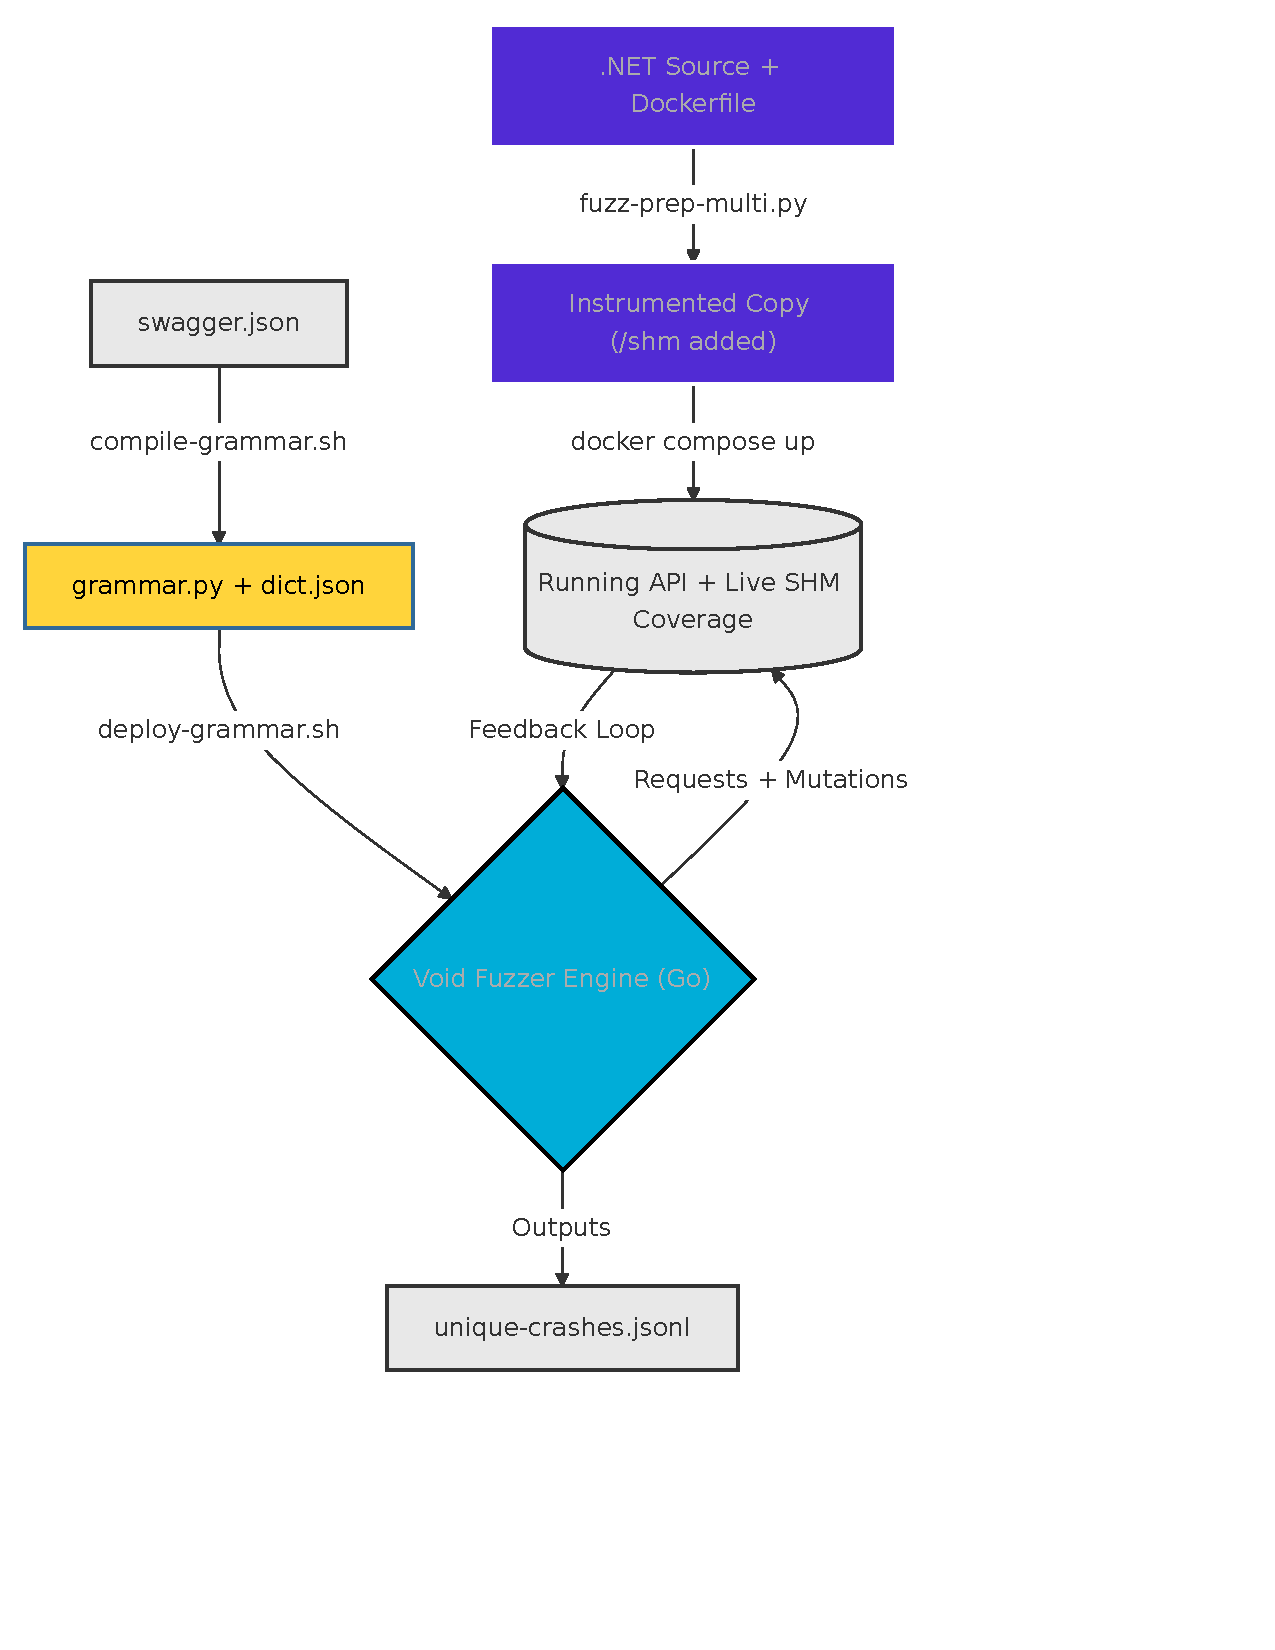
\includegraphics[width=\linewidth]{architecture.pdf}}
\caption{UpsideFuzzer end-to-end pipeline. The preparation phase (left) produces an instrumented Docker image and enhanced grammar. The fuzzing phase (right) runs the Void engine against the instrumented target.}
\label{fig:architecture}
\end{figure}

\textbf{Preparation phase (run once per target):}
\begin{enumerate}
    \item Run \texttt{fuzz-prep-multi.py} to instrument the application Docker image.
    \item Run \texttt{compile-grammar.sh} to generate grammar from the OpenAPI specification, then enhance it with source-derived values.
\end{enumerate}

\textbf{Fuzzing phase (the actual test run):}
\begin{enumerate}
    \item The Void runtime engine sends requests from the grammar to the instrumented application.
    \item It reads code-coverage feedback from the target.
    \item It uses the feedback to decide what to try next.
\end{enumerate}

The following subsections describe each component in detail.

% ============================================================
\subsection{Grammar Construction: From OpenAPI to Typed Templates}
\label{sec:grammar_model}
% ============================================================

The fuzzer does not send arbitrary HTTP requests. Instead, every request is built from a \textbf{template} derived from the OpenAPI specification. A template is a skeleton of a valid HTTP request with ``holes'' (slots) where the fuzzer inserts values.

Each template contains three kinds of segments:
\begin{itemize}
    \item \textbf{Static segments:} fixed parts copied verbatim --- HTTP method, path delimiters, header names, JSON keys.
    \item \textbf{Fuzzable segments:} typed placeholders (\texttt{string}, \texttt{int}, \texttt{uuid}, \texttt{datetime}, etc.) where the fuzzer inserts or mutates values from the dictionary.
    \item \textbf{Custom-payload segments:} dependency slots filled with values learned at runtime from earlier responses (e.g., a server-generated ID or token).
\end{itemize}

\textbf{Example.} Consider a simple endpoint:
\begin{lstlisting}
POST /api/orders/{orderId}/lines
Content-Type: application/json

{"sku": "...", "quantity": 1}
\end{lstlisting}

The grammar compiler converts this into:
\begin{lstlisting}
template: post_order_line
segments:
  [static]  "POST /api/orders/"
  [dynamic] orderId  (from earlier response)
  [static]  "/lines HTTP/1.1\r\n..."
  [static]  "{\"sku\":"
  [fuzzable:string] sku
  [static]  ",\"quantity\":"
  [fuzzable:int]    quantity
  [static]  "}"
reads:  [orderId]
writes: []
\end{lstlisting}

This means the fuzzer \emph{always} sends a syntactically valid HTTP request with correct JSON. It only changes the values in the typed slots. This is the key difference from byte-level mutation: the request structure is never broken.

The \texttt{reads} and \texttt{writes} annotations, recovered by RESTler's compiler, tell the fuzzer about dependencies between endpoints: which requests produce values and which consume them.

% ============================================================
\subsection{Semantic Source Extraction (SSE): Making the Dictionary Smarter}
\label{sec:sse}
% ============================================================

\begin{figure}[htbp]
\centerline{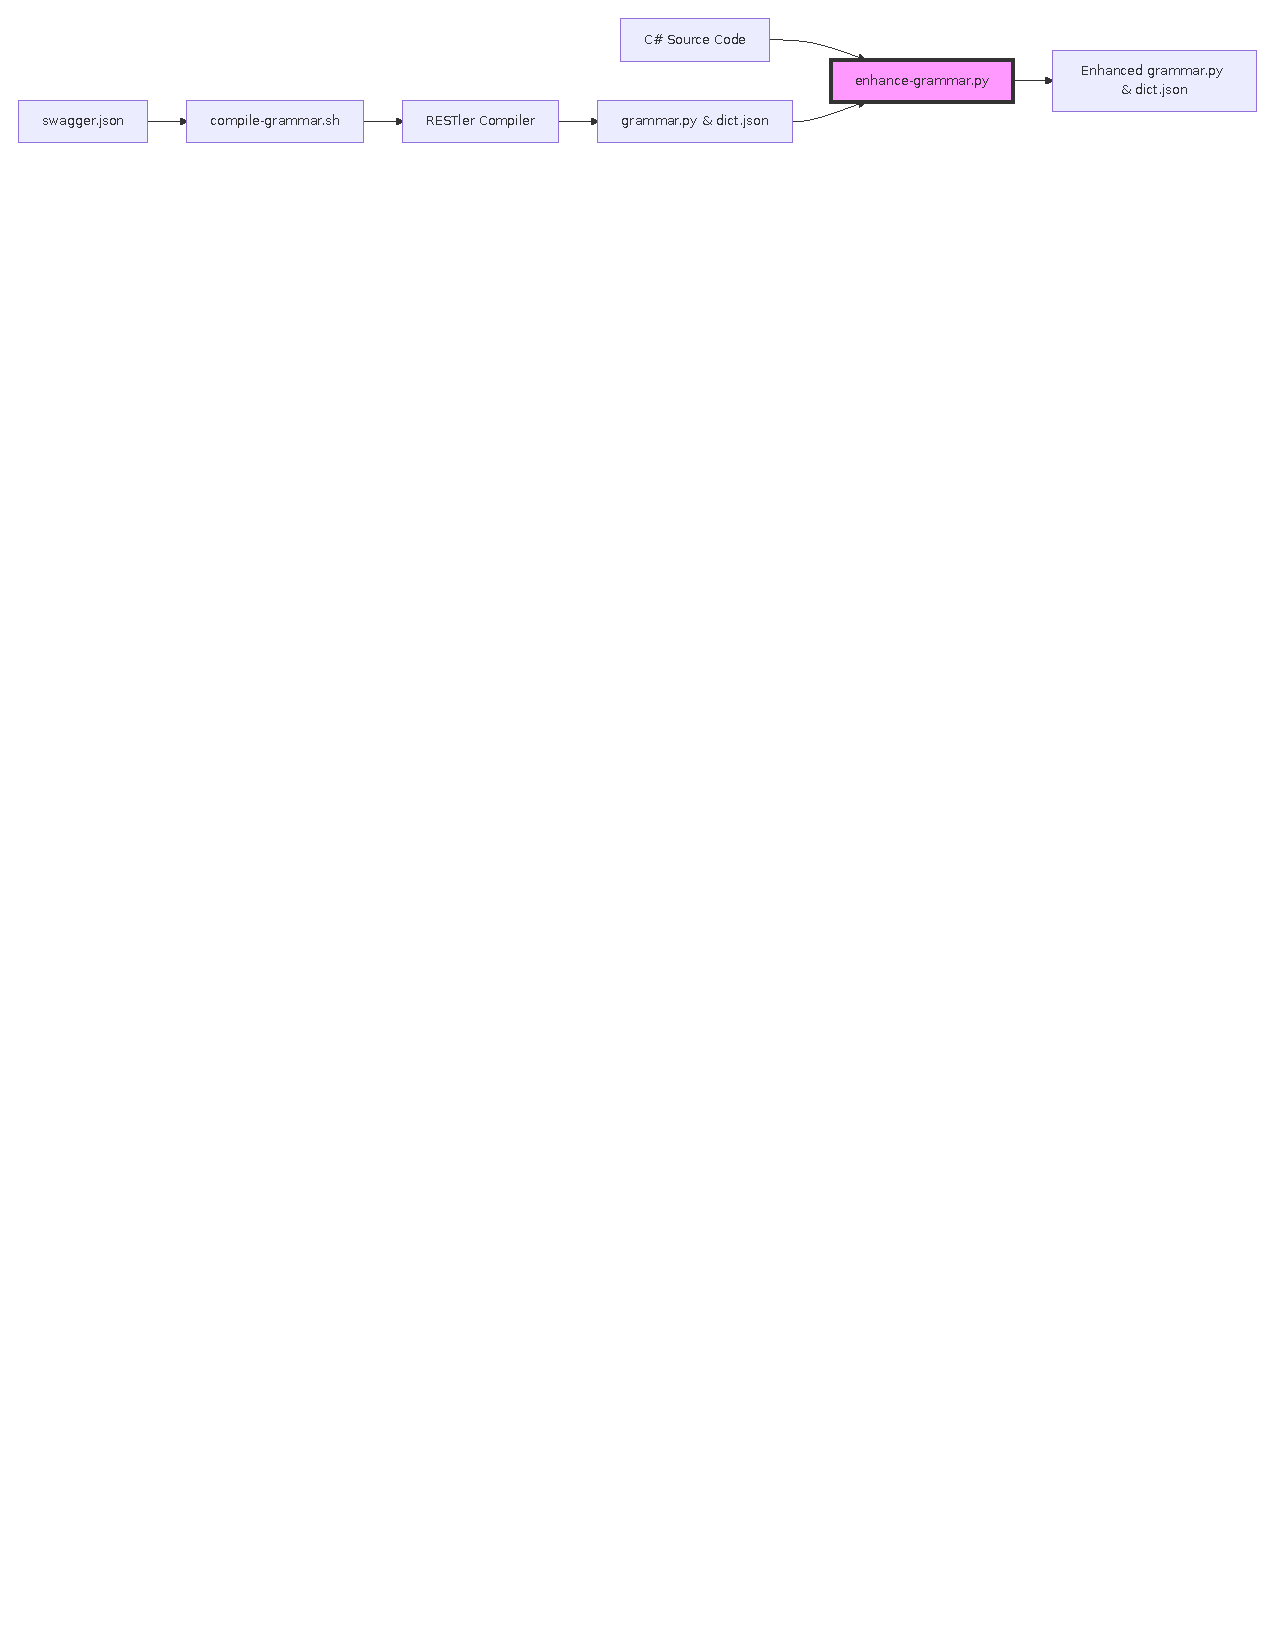
\includegraphics[width=\linewidth]{sse.pdf}}
\caption{Semantic Source Extraction pipeline. The enhancer reads constraints from both the OpenAPI specification and C\# source code, then inserts boundary-focused values into the RESTler dictionary.}
\label{fig:sse}
\end{figure}

\subsubsection{The Problem SSE Solves}

Consider a REST API field with the following C\# validation:
\begin{lstlisting}
[StringLength(8, MinimumLength = 4)]
public string Username { get; set; }
\end{lstlisting}

RESTler's default dictionary contains the value \texttt{"fuzzstring"} (10 characters), which immediately fails this validation. The request is rejected, and the fuzzer never reaches the code that actually processes the username. SSE solves this by reading the validation rule directly from the source code and generating values that are designed to test the boundaries: strings of length 3 (below minimum), 4 (at minimum), 8 (at maximum), and 9 (above maximum).

\subsubsection{Two Sources of Constraints}

SSE reads constraints from two places:

\textbf{1. OpenAPI specification:} fields like \texttt{minLength}, \texttt{maxLength}, \texttt{minimum}, \texttt{maximum}, \texttt{pattern}, and \texttt{enum} declared in the Swagger/OpenAPI JSON.

\textbf{2. C\# source code:} the enhancer scans all \texttt{.cs} files in the project and recognizes two common validation frameworks:

\begin{itemize}
    \item \textbf{Data Annotations:} attributes like \texttt{[StringLength]}, \texttt{[Range]}, \texttt{[Required]}, \texttt{[MaxLength]}, \texttt{[MinLength]}, \texttt{[RegularExpression]}, \texttt{[EmailAddress]}, \texttt{[Url]}.
    \item \textbf{FluentValidation:} method chains like \texttt{.MaximumLength(N)}, \texttt{.InclusiveBetween(lo, hi)}, \texttt{.GreaterThan(v)}, \texttt{.Matches("pattern")}, \texttt{.NotEmpty()}.
\end{itemize}

When the same field has constraints in both the specification and the source code, SSE keeps the tighter (more restrictive) constraint.

\textbf{Enum resolution.} For fields whose type is a C\# \texttt{enum}, the extractor locates the enum declaration, parses all member names and their integer values, and adds both forms to the dictionary. This is important because many APIs reject any value outside the defined enum set.

\subsubsection{Boundary Value Synthesis}

Given the extracted constraints, SSE generates a small set of targeted test values. The strategy is simple and follows classical boundary-value analysis:

\begin{algorithm}[t]
\caption{Boundary Value Synthesis}
\label{alg:boundary}
\begin{algorithmic}[1]
\REQUIRE Field constraint $F$ with type, min, max, pattern
\STATE values $\leftarrow \{\}$
\IF{$F$ is numeric with range $[lo, hi]$}
    \STATE values $\leftarrow \{lo-1,\; lo,\; hi,\; hi+1\}$
\ELSIF{$F$ is string with length $[minLen, maxLen]$}
    \STATE values $\leftarrow \{$str of len $minLen-1$, $minLen$, $maxLen$, $maxLen+1\}$
\ELSIF{$F$ has regex pattern $p$}
    \STATE values $\leftarrow \{$one matching example, one non-matching$\}$
\ENDIF
\IF{$F$ has enum members $\{e_1, \ldots, e_n\}$}
    \STATE values $\leftarrow$ values $\cup$ all enum names and numeric equivalents
\ENDIF
\STATE Insert values into dictionary under field name variants
\STATE \quad (camelCase, PascalCase, lowercase)
\RETURN values
\end{algorithmic}
\end{algorithm}

\textbf{Important:} SSE does not modify RESTler's grammar structure or compiler. It only enriches the \emph{dictionary} with better values and, when needed, adds seed templates for endpoints that the compiler cannot handle (such as multipart file-upload endpoints).

% ============================================================
\subsection{Automated Instrumentation Pipeline}
\label{sec:instrumentation}
% ============================================================

\subsubsection{What Is Instrumentation?}

In the context of fuzzing, \textbf{instrumentation} means inserting small pieces of code into the target program that record which parts of the code were executed during a request. Think of it as placing sensors at every branch point in the code: ``if the program took the left branch, increment counter~A; if it took the right branch, increment counter~B.'' After processing a request, the fuzzer reads these counters to see which code paths were exercised.

For .NET applications, UpsideFuzzer uses SharpFuzz~\cite{sharpfuzz}, which rewrites compiled \texttt{.dll} files at the Intermediate Language (IL) level. SharpFuzz inserts a counter at each branch edge using the following mechanism:

\begin{equation}
  \text{bitmap}[(\text{prev\_block} \oplus \text{cur\_block})] \mathrel{+}= 1
  \label{eq:shm}
\end{equation}

Here, \texttt{prev\_block} and \texttt{cur\_block} are random identifiers assigned to basic blocks in the code, and $\oplus$ is the XOR operation. The result indexes into a 65,536-byte shared-memory bitmap. This is the same approach used by AFL~\cite{afl}. Each byte in the bitmap represents one \emph{edge} (a transition between two blocks). A non-zero value means ``this edge was executed at least once.''

\subsubsection{The 4-Stage Docker Build}

UpsideFuzzer instruments the target application automatically during the Docker build, without requiring any manual harness code. The preparation script \texttt{fuzz-prep-multi.py} modifies the Dockerfile to add four stages:

\begin{algorithm}[t]
\caption{Automated Instrumentation Pipeline}
\label{alg:instrument}
\begin{algorithmic}[1]
\REQUIRE Target repository with Dockerfile
\STATE \textbf{Stage 1 (builder):} Build the instrumentor tool from source
\STATE \textbf{Stage 2 (publish):} Run \texttt{dotnet publish} as usual
\STATE \textbf{Stage 3 (instrument):}
\FORALL{DLL files in published output}
    \IF{DLL namespace matches detected business logic}
        \STATE Rewrite IL with SharpFuzz edge counters
    \ENDIF
\ENDFOR
\STATE \textbf{Stage 4 (runtime):} Copy instrumented binaries to final image
\STATE Patch \texttt{Program.cs} to expose coverage over HTTP
\STATE Update \texttt{docker-compose.yaml} for shared memory
\end{algorithmic}
\end{algorithm}

\textbf{Namespace filtering.} Not every DLL in a .NET application should be instrumented. System libraries, Entity Framework migrations, and auto-generated code would add noise without useful coverage signal. The script detects business-logic namespaces by scanning for files matching patterns like \texttt{*Controller.cs}, \texttt{*Service.cs}, \texttt{*Validator.cs}, and \texttt{*Handler.cs}. Only code in these namespaces gets instrumented.

\subsubsection{Coverage Transport: Two Modes}

The instrumented .NET process writes coverage data into a shared-memory bitmap. UpsideFuzzer reads this bitmap in two ways:

\begin{enumerate}
    \item \textbf{Direct SHM mode (fastest):} The fuzzer container and the application container share a \texttt{tmpfs} volume. The fuzzer reads the bitmap directly from memory, with near-zero overhead.
    \item \textbf{HTTP mode (fallback):} The patched application exposes HTTP endpoints (\texttt{/shm/coverage}, \texttt{/shm/reset}) that return the coverage data as JSON. This works in any Docker setup but adds a small network overhead.
\end{enumerate}

In both modes, the practical result is the same: after each request (or batch of requests), the fuzzer knows how many new code edges were discovered.

% ============================================================
\section{The Full Fuzzing Cycle and Feedback Loop}
\label{sec:void}
% ============================================================

\subsection{The Void Execution Engine}

Void is the runtime component of UpsideFuzzer --- a concurrent HTTP fuzzing engine written in Go (~3,500 lines). It reads the grammar templates and dictionary, sends requests to the instrumented .NET application, collects coverage feedback, and uses it to guide future requests.

\subsection{Step-by-Step Cycle}
\label{sec:feedback_loop}

The core of Void is a feedback loop that repeats the following five steps for the entire duration of the fuzzing campaign (Figure~\ref{fig:feedbackloop}):

\begin{enumerate}
    \item \textbf{Pick a seed.} Choose a previously successful request from the corpus. Requests that discovered more new code get chosen more often.
    \item \textbf{Build a request.} Take the template associated with the seed, fill in the slot values: copy static parts, plug in learned IDs for dependency slots, pick or mutate values for fuzzable slots from the dictionary.
    \item \textbf{Send the request.} Execute the rendered HTTP request against the instrumented target. Record the response status code, body, and latency.
    \item \textbf{Measure coverage.} Read the coverage bitmap to count how many \emph{new} edges this request (or batch) discovered. A new edge means the request executed code that no previous request had reached.
    \item \textbf{Update state.} If new edges were found: save this request as a new seed with high priority, record which mutation type worked, and reset the stall counter. If no new edges: increment the stall counter; after too many stalls, switch to more aggressive mutations.
\end{enumerate}

\begin{figure}[t]
\centering
\resizebox{\columnwidth}{!}{%
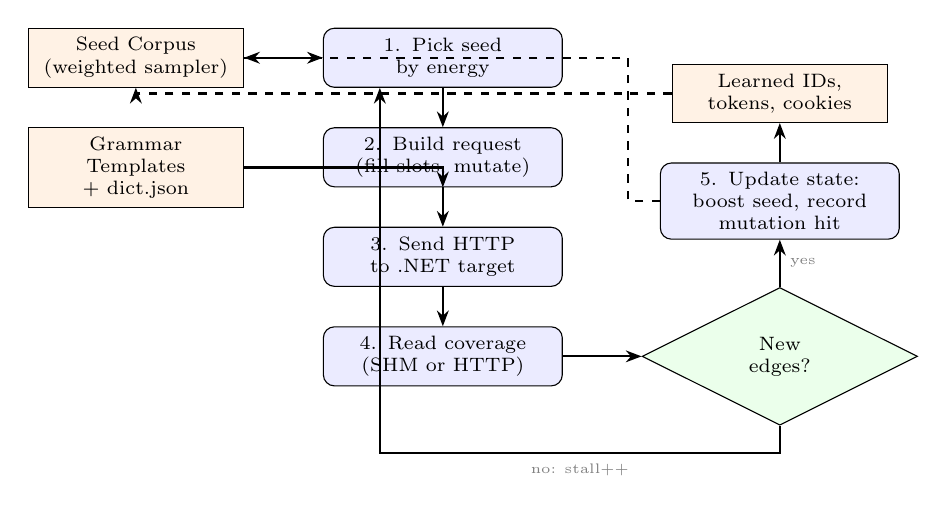
\begin{tikzpicture}[
    node distance=0.9cm and 0.4cm,
    block/.style={rectangle, draw, rounded corners, fill=blue!8,
                  text width=2.8cm, minimum height=0.75cm, align=center,
                  font=\scriptsize},
    data/.style={rectangle, draw, fill=orange!10, text width=2.5cm,
                 minimum height=0.6cm, align=center, font=\scriptsize},
    decision/.style={diamond, draw, fill=green!8, aspect=2,
                     text width=1.8cm, align=center, font=\scriptsize},
    arr/.style={-{Stealth[length=2mm]}, thick},
    lab/.style={font=\tiny, text=gray},
]
% Left column: inputs
\node[data] (corpus) {Seed Corpus\\(weighted sampler)};
\node[data, below=0.5cm of corpus] (grammar) {Grammar Templates\\+ dict.json};

% Center column: processing
\node[block, right=1.0cm of corpus] (select) {1. Pick seed\\by energy};
\node[block, below=0.5cm of select] (render) {2. Build request\\(fill slots, mutate)};
\node[block, below=0.5cm of render] (send) {3. Send HTTP\\to .NET target};
\node[block, below=0.5cm of send] (measure) {4. Read coverage\\(SHM or HTTP)};

% Right column: feedback
\node[decision, right=1.0cm of measure] (novel) {New\\edges?};
\node[block, above=0.6cm of novel] (update) {5. Update state:\\boost seed, record\\mutation hit};
\node[data, above=0.5cm of update] (learn) {Learned IDs,\\tokens, cookies};

% Arrows: main flow
\draw[arr] (corpus) -- (select);
\draw[arr] (grammar) -| (render);
\draw[arr] (select) -- (render);
\draw[arr] (render) -- (send);
\draw[arr] (send) -- (measure);
\draw[arr] (measure) -- (novel);

% Arrows: feedback path
\draw[arr] (novel) -- node[right, lab] {yes} (update);
\draw[arr] (update) -- (learn);
\draw[arr, dashed] (learn) -| (corpus);
\draw[arr, dashed] (update.west) -- ++(-0.4,0) |- (corpus.east);

% No-edge path
\draw[arr] (novel.south) -- ++(0,-0.35) -| node[below, lab, pos=0.25] {no: stall++} ([xshift=-0.8cm]select.south);

\end{tikzpicture}
}
\caption{Void's coverage-guided feedback loop. Solid arrows show data flow within one iteration; dashed arrows show feedback that changes future iterations.}
\label{fig:feedbackloop}
\end{figure}

\subsection{Simplified Pseudocode for the Main Loop}

Algorithm~\ref{alg:feedback} shows the main fuzzing loop in simplified form. The three key decisions are: which seed to pick, how to read coverage, and how to update priorities when something interesting is found.

\begin{algorithm}[t]
\caption{Coverage-Guided Fuzzing Loop (Simplified)}
\label{alg:feedback}
\begin{algorithmic}[1]
\REQUIRE Templates $T$, dictionary $D$, time budget $B$
\STATE corpus $\leftarrow$ send each template unmutated, save results
\STATE edges $\leftarrow$ initial edge count; stall $\leftarrow 0$
\WHILE{elapsed $< B$}
    \STATE seed $\leftarrow$ pick from corpus (higher energy = more likely)
    \STATE template $\leftarrow$ seed's template
    \STATE request $\leftarrow$ render(template, $D$, learned\_values)
    \STATE response $\leftarrow$ sendHTTP(request)
    \STATE new\_edges $\leftarrow$ measureCoverage() $-$ edges
    \IF{new\_edges $> 0$}
        \STATE edges $\leftarrow$ edges $+$ new\_edges
        \STATE add request to corpus with energy $\propto$ new\_edges
        \STATE boost parent seed's energy
        \STATE record which mutation category found new code
        \STATE stall $\leftarrow 0$
    \ELSE
        \STATE stall $\leftarrow$ stall $+ 1$
    \ENDIF
    \STATE learnValues(response)  \COMMENT{extract IDs, tokens}
    \IF{stall too high}
        \STATE switch to more aggressive mutations
    \ENDIF
\ENDWHILE
\end{algorithmic}
\end{algorithm}

\subsection{How Coverage Feedback Steers the Search}
\label{sec:coverage_influence}

When Void discovers that a request reached new code, the feedback updates three independent aspects of the mutation pipeline (Figure~\ref{fig:cov_influence}):

\textbf{1. Seed energy.} Requests that found new edges become seeds with higher ``energy,'' meaning they get picked more often in future iterations. Every time a seed is picked, its energy decreases by 0.5\%, so no single seed dominates forever.

\textbf{2. Endpoint weight.} Each API endpoint (e.g., \texttt{POST /api/users}) has a health score. Endpoints that keep producing new coverage keep their weight. Endpoints that only return errors or repeat the same code lose weight and get picked less often.

\textbf{3. Mutation category weight.} UpsideFuzzer organizes mutation payloads into 15 categories (see Section~\ref{sec:mutations}). Each category's selection probability is updated based on its success rate:

\begin{equation}
  \text{category\_weight} = 1 + 4 \times \frac{\text{hits}}{\text{attempts}}
  \label{eq:mutcat_weight}
\end{equation}

This means a mutation family that keeps finding new code can become up to $5\times$ more likely to be selected than one that never does. This adaptive approach follows the MOpt~\cite{mopt} scheduling strategy.

\begin{figure}[t]
\centering
\resizebox{\columnwidth}{!}{%
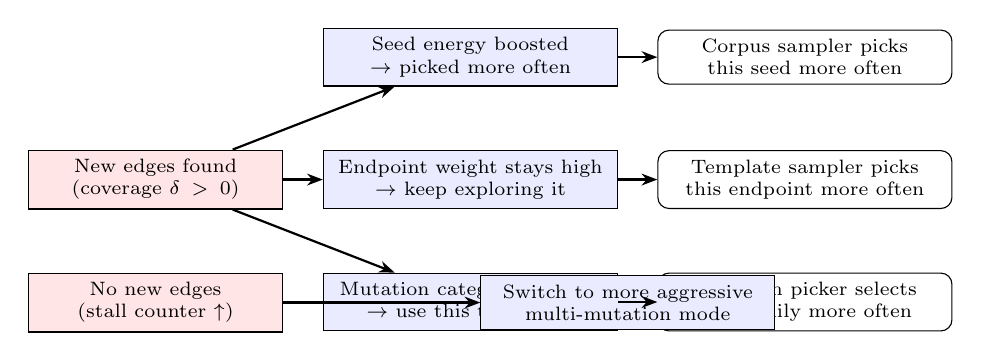
\begin{tikzpicture}[
    node distance=0.7cm,
    box/.style={rectangle, draw, rounded corners, text width=3.5cm,
                minimum height=0.65cm, align=center, font=\scriptsize},
    signal/.style={rectangle, draw, fill=red!10, text width=3.0cm,
                   minimum height=0.6cm, align=center, font=\scriptsize},
    effect/.style={rectangle, draw, fill=blue!8, text width=3.5cm,
                   minimum height=0.6cm, align=center, font=\scriptsize},
    arr/.style={-{Stealth[length=2mm]}, thick},
]
% Central signal
\node[signal] (delta) {New edges found\\(coverage $\delta > 0$)};

% Three effects
\node[effect, above right=0.8cm and 0.5cm of delta] (seed)
    {Seed energy boosted\\$\rightarrow$ picked more often};
\node[effect, right=0.5cm of delta] (endpoint)
    {Endpoint weight stays high\\$\rightarrow$ keep exploring it};
\node[effect, below right=0.8cm and 0.5cm of delta] (mopt)
    {Mutation category boosted\\$\rightarrow$ use this type more};

% Downstream effects
\node[box, right=0.5cm of seed] (fenwick) {Corpus sampler picks\\this seed more often};
\node[box, right=0.5cm of endpoint] (tmpl) {Template sampler picks\\this endpoint more often};
\node[box, right=0.5cm of mopt] (cat) {Mutation picker selects\\this family more often};

% Anti-stagnation
\node[signal, below=0.8cm of delta] (stall)
    {No new edges\\(stall counter $\uparrow$)};
\node[effect, right=2.5cm of stall] (havoc) {Switch to more aggressive\\multi-mutation mode};

% Arrows
\draw[arr] (delta) -- (seed);
\draw[arr] (delta) -- (endpoint);
\draw[arr] (delta) -- (mopt);
\draw[arr] (seed) -- (fenwick);
\draw[arr] (endpoint) -- (tmpl);
\draw[arr] (mopt) -- (cat);
\draw[arr] (stall) -- (havoc);

\end{tikzpicture}
}
\caption{How coverage feedback influences the mutation pipeline. A positive edge delta boosts three independent weights. Persistent lack of new edges escalates mutation aggressiveness.}
\label{fig:cov_influence}
\end{figure}

\subsection{Dynamic Value Learning and Stateful Execution}
\label{sec:state}

Many API workflows require state: a \texttt{POST} creates a resource and returns an ID, and later \texttt{GET}, \texttt{PUT}, and \texttt{DELETE} requests must reuse that ID. Void handles this by scanning successful responses for values like IDs, tokens, anti-forgery fields, and session cookies. These learned values are stored and automatically replayed into later requests that depend on them. When a template needs a \texttt{custom\_payload} value, the renderer first tries learned values, then falls back to the static dictionary.

% ============================================================
\section{Fuzzer Capabilities and Configuration}
\label{sec:capabilities}
% ============================================================

\subsection{Epochs: Five Phases of a Fuzzing Campaign}
\label{sec:phases}

Void divides a fuzzing run into five sequential phases, each with a different objective. Table~\ref{tab:epochs} shows the default time allocation.

\begin{table}[htbp]
\caption{Void Fuzzing Campaign Epochs}
\label{tab:epochs}
\centering
\footnotesize
\setlength{\tabcolsep}{4pt}
\resizebox{\columnwidth}{!}{%
\begin{tabular}{llrl}
\toprule
\textbf{Epoch} & \textbf{Strategy} & \textbf{Budget} & \textbf{Purpose} \\
\midrule
Baseline      & No mutation    & 5\%  & Send every template as-is to establish \\
              &                &      & coverage baseline and populate corpus \\
\midrule
Harvest       & Light mutation & 25\% & Focus on getting 2xx responses to \\
              &                &      & learn IDs, tokens, and session state \\
\midrule
Deterministic & Single mutation& 25\% & Systematic boundary-value substitution, \\
              &                &      & one field at a time \\
\midrule
Havoc         & Multi-mutation & 35\% & Random combinations of 1--4 stacked \\
              &                &      & mutations per request \\
\midrule
Splicing      & Cross-seed     & 10\% & Combine parts of two previously \\
              &                &      & successful seeds into new requests \\
\bottomrule
\end{tabular}
}
\end{table}

The key idea: start simple (send valid requests, learn the API's dynamic values), then get progressively more aggressive with mutations. At each phase transition, Void checks how much progress was made. If the current phase is stalling, the remaining time is shifted to the Havoc phase, which is better at broad exploration.

\subsection{Key Configuration Settings}
\label{sec:settings}

UpsideFuzzer is designed to work out of the box with sensible defaults. The most important user-facing settings are:

\begin{table}[htbp]
\caption{Key Fuzzer Settings}
\label{tab:settings}
\centering
\footnotesize
\setlength{\tabcolsep}{4pt}
\resizebox{\columnwidth}{!}{%
\begin{tabular}{llp{4.5cm}}
\toprule
\textbf{Flag} & \textbf{Default} & \textbf{What It Controls} \\
\midrule
\texttt{-time-budget}      & 10 min  & Total fuzzing duration \\
\texttt{-concurrency}      & 10      & Number of parallel HTTP workers \\
\texttt{-direct-shm}       & false   & Use direct shared-memory coverage (fastest) \\
\texttt{-sequence-prob}     & 0.30    & Probability of building multi-step sequences \\
\texttt{-skip-endpoint-on-500} & false & Stop fuzzing an endpoint after first crash \\
\texttt{-crash-triage}      & true    & Verify and minimize crashes automatically \\
\bottomrule
\end{tabular}
}
\end{table}

\textbf{Adaptive concurrency.} Void automatically adjusts the number of parallel workers during a run. If the target responds quickly without errors, Void increases concurrency, applying principles similar to TCP congestion control. If latency spikes or error rates increase, it backs off. This prevents overwhelming the target while maximizing throughput.

\subsection{Structured Mutation Operators}
\label{sec:mutations}

Unlike byte-level fuzzers, Void mutates requests in a \emph{type-aware} way. Integers stay integers, UUIDs keep their shape, and JSON stays parseable. For string fields, Void uses 15 categories of security-focused payloads, each targeting a common vulnerability class:

\begin{table}[htbp]
\caption{Mutation Categories with Adaptive Weights}
\label{tab:mutation_cats}
\centering
\footnotesize
\setlength{\tabcolsep}{3pt}
\resizebox{\columnwidth}{!}{%
\begin{tabular}{llp{4.0cm}}
\toprule
\textbf{Category} & \textbf{Base Weight} & \textbf{Example Payloads} \\
\midrule
boundary    & 1.0 & \texttt{""}, \texttt{null}, \texttt{NaN} \\
overflow    & 1.0 & Long strings (100--10000 chars) \\
sqli        & 1.5 & \texttt{' OR '1'='1}, \texttt{UNION SELECT} \\
xss         & 1.5 & \texttt{<script>alert(1)</script>} \\
cmdi        & 1.5 & \texttt{; id}, \texttt{\$(id)} \\
path\_trav.  & 1.5 & \texttt{../../../etc/passwd} \\
ssrf        & 1.5 & AWS/GCP metadata URLs \\
ssti        & 1.5 & \texttt{\{\{7*7\}\}}, \texttt{\$\{7*7\}} \\
crlf        & 1.0 & \texttt{\textbackslash r\textbackslash nX-Injected: pwned} \\
open\_redir  & 1.0 & \texttt{//evil.com} \\
log4shell   & 1.0 & \texttt{\$\{jndi:ldap://...\}} \\
nosqli      & 1.0 & \texttt{\{"\$gt":""\}} \\
ldap        & 1.0 & \texttt{*)(uid=*} \\
xxe         & 1.0 & \texttt{<!DOCTYPE foo [<!ENTITY xxe ...>]>} \\
unicode     & 1.0 & Zero-width chars, BOM, RTL markers \\
\bottomrule
\end{tabular}
}
\end{table}

Categories that find new code edges have their weight increased automatically (Equation~\ref{eq:mutcat_weight}). Over a long campaign, the fuzzer naturally focuses on mutation types that are productive for the specific target.

\textbf{Structured body havoc.} For JSON bodies, Void also applies structural mutations: removing fields, duplicating fields, changing value types, inserting nulls, or combining fragments from different seeds. The JSON structure is always kept valid. Path mutation is limited to segments that look like resource identifiers, so the route shape remains correct.

% ============================================================
\section{Evaluation}
\label{sec:eval}
% ============================================================

\subsection{Research Questions}
\begin{itemize}
    \item \textbf{RQ1}: Does source-derived grammar enhancement improve the fuzzer's ability to bypass validation and reach deeper code?
    \item \textbf{RQ2}: Does the coverage-guided loop find more code paths and crashes than the black-box baseline?
    \item \textbf{RQ3}: How does UpsideFuzzer perform on internal production-grade microservices?
\end{itemize}

\subsection{Experimental Setup}

All experiments were run on identical hardware: 8-core CPU, 16 GB RAM, no network throttling. We compare two configurations:
\begin{itemize}
    \item \textbf{RESTler baseline}: RESTler Fuzz mode with default dictionary, no SSE, no coverage feedback.
    \item \textbf{UpsideFuzzer}: full pipeline with SSE-augmented grammar and Void coverage-guided loop.
\end{itemize}

% -----------------------------------------------------------
\subsection{24-Hour Evaluation on Three Applications}
\label{sec:eval_24h}
% -----------------------------------------------------------

We ran 24-hour campaigns on three .NET REST API applications:
\begin{itemize}
    \item \textbf{nopCommerce}: open-source e-commerce platform ($\sim$180K LoC, 200+ endpoints, extensive Data Annotation and FluentValidation).
    \item \textbf{eShopOnContainers}: Microsoft's reference microservice architecture ($\sim$70K LoC, 6 services, 100+ endpoints).
    \item \textbf{mpt-helpdesk}: custom enterprise helpdesk API ($\sim$25K LoC, 60+ endpoints, complex role-based authorization).
\end{itemize}

Table~\ref{tab:results} and Figure~\ref{fig:eval24hplots} show the results.

\begin{table}[htbp]
\caption{24-Hour Fuzzing Results: RESTler vs.\ UpsideFuzzer}
\label{tab:results}
\centering
\footnotesize
\setlength{\tabcolsep}{4pt}
\resizebox{\columnwidth}{!}{%
\begin{tabular}{llrrl}
\toprule
\textbf{Target} & \textbf{Tool} & \textbf{Edges} & \textbf{5xx Found} & \textbf{TTFC}$^{a}$ \\
\midrule
\multirow{2}{*}{nopCommerce}
  & RESTler     & 5,430  & 2  & 4h 15m \\
  & \textbf{UpsideFuzzer} & \textbf{12,850}$^{+136\%}$ & \textbf{14} & \textbf{0h 45m} \\
\midrule
\multirow{2}{*}{eShopOnCont.}
  & RESTler     & 3,120  & 0  & N/A \\
  & \textbf{UpsideFuzzer} & \textbf{8,400}$^{+169\%}$ & \textbf{3} & \textbf{2h 10m} \\
\midrule
\multirow{2}{*}{mpt-helpdesk}
  & RESTler     & 1,850  & 1  & 8h 30m \\
  & \textbf{UpsideFuzzer} & \textbf{4,200}$^{+127\%}$ & \textbf{7} & \textbf{1h 20m} \\
\bottomrule
\end{tabular}
}
\vspace{2pt}
\footnotesize{$^{a}$Time to First Crash (5xx response). N/A means no crashes were found.}
\end{table}

\begin{figure*}[t]
\centering
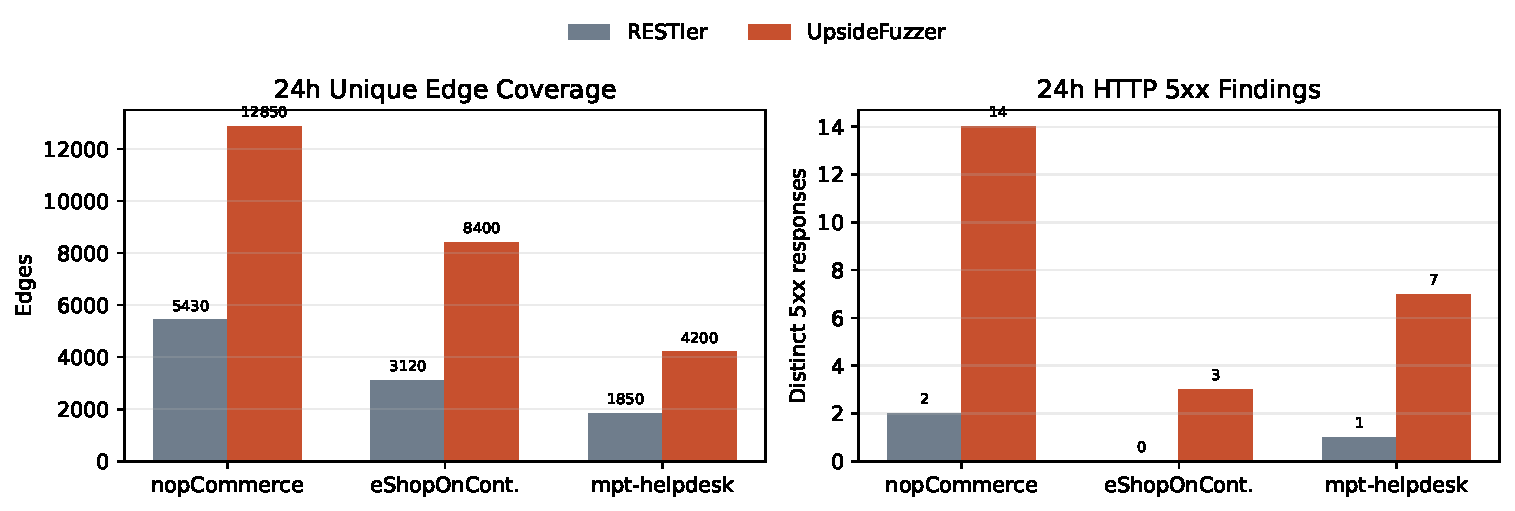
\includegraphics[width=0.97\textwidth]{figures/eval_24h_overview.pdf}
\caption{24-hour evaluation results. Left: unique branch edges discovered. Right: distinct HTTP 5xx responses found. UpsideFuzzer consistently outperforms the RESTler baseline on all targets.}
\label{fig:eval24hplots}
\end{figure*}

\textbf{Key observations:}
\begin{itemize}
    \item UpsideFuzzer covers $127\%$--$169\%$ more unique code edges than RESTler across all three targets.
    \item On eShopOnContainers, RESTler finds zero crashes. Without semantically valid enum and integer values, every mutated request is rejected at the FluentValidation layer. UpsideFuzzer's SSE pass recovers 12 enum types and 8 numeric ranges from the source, enabling it to break through validation and discover 3 service crashes.
    \item Time to First Crash is $3\times$--$6\times$ faster with UpsideFuzzer.
\end{itemize}

% -----------------------------------------------------------
\subsection{20-Minute Reproducible Docker Benchmark}
\label{sec:eval_docker}
% -----------------------------------------------------------

To provide a reproducible comparison, we ran a 20-minute benchmark on four public .NET services in Docker. Both tools used the same grammars and authentication tokens. Table~\ref{tab:dockerbench} and Figure~\ref{fig:dockerplots} show the results.

\begin{table}[htbp]
\caption{Reproducible 20-Minute Docker Benchmark}
\label{tab:dockerbench}
\centering
\footnotesize
\setlength{\tabcolsep}{3.5pt}
\resizebox{\columnwidth}{!}{%
\begin{tabular}{llrrrl}
\toprule
\textbf{Target} & \textbf{Tool} & \textbf{OpenAPI Cov.} & \textbf{Requests} & \textbf{500 M+E}$^{a}$ & \textbf{Feedback} \\
\midrule
\multirow{2}{*}{eShopOnWeb}
  & RESTler & 6/8 & 899 & 1 & Spec-guided \\
  & Void & 6/8 & \textbf{4,423,205} & \textbf{2} & 660 edges \\
\midrule
\multirow{2}{*}{CustomerLoyalty}
  & RESTler & 3/3 & 116,853 & 1 & Spec-guided \\
  & Void & 3/3 & \textbf{4,580,149} & 1 & 38,150 edges \\
\midrule
\multirow{2}{*}{Catalog.API}
  & RESTler & 10/12 & 148,566 & \textbf{12} & Spec-guided \\
  & Void & 11/12 & \textbf{6,616,420} & 8 & 154 edges \\
\midrule
\multirow{2}{*}{Jellyfin}
  & RESTler & 190/309 & 58,407 & 18 & Spec-guided \\
  & Void & \textbf{309/309} & \textbf{4,941,012} & \textbf{97} & 152,567 edges \\
\bottomrule
\end{tabular}
}
\vspace{2pt}
\footnotesize{$^{a}$Distinct HTTP 500-producing method+endpoint pairs.}
\end{table}

\begin{figure*}[t]
\centering
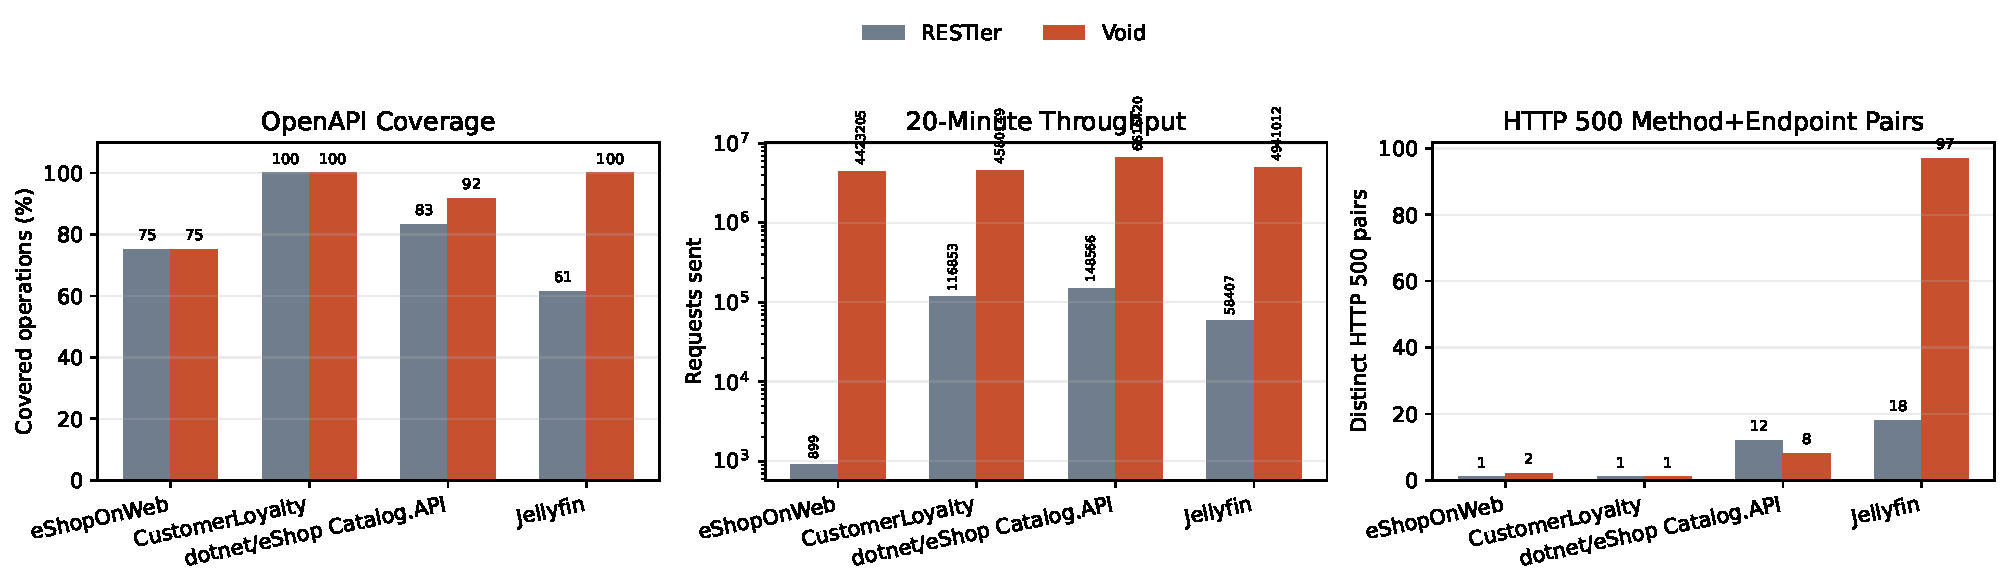
\includegraphics[width=\textwidth]{figures/docker_benchmark_overview.pdf}
\caption{20-minute Docker benchmark results. Left: OpenAPI operation coverage. Middle: request throughput (log scale). Right: distinct HTTP 500 method+endpoint pairs.}
\label{fig:dockerplots}
\end{figure*}

\textbf{Key observations:}
\begin{itemize}
    \item \textbf{Coverage:} Void matches or exceeds RESTler's OpenAPI coverage on all four targets. On Jellyfin, Void reaches full 309/309 endpoint coverage vs.\ RESTler's 190/309.
    \item \textbf{Throughput:} Void sends $39\times$--$85\times$ more requests than RESTler due to its concurrent Go architecture.
    \item \textbf{Bug finding:} Aggregated over all four targets, Void discovers 108 distinct HTTP 500 method+endpoint pairs vs.\ 32 for RESTler. RESTler finds more 500s on Catalog.API specifically, showing that specification-guided exploration can find certain classes of bugs efficiently.
\end{itemize}

% -----------------------------------------------------------
\subsection{Internal Microservice Evaluation}
\label{sec:eval_internal}
% -----------------------------------------------------------

To validate UpsideFuzzer's applicability to production-grade enterprise systems, we ran the same 24-hour comparison on five internal .NET microservices. These services are representative of typical enterprise API workloads: they use SQL Server, Azure Service Bus, Blob Storage, and complex role-based authorization. Table~\ref{tab:internal} shows the results. Service names are anonymized for confidentiality.

\begin{table}[htbp]
\caption{24-Hour Results on Internal Enterprise Microservices}
\label{tab:internal}
\centering
\footnotesize
\setlength{\tabcolsep}{3.5pt}
\resizebox{\columnwidth}{!}{%
\begin{tabular}{llrrrl}
\toprule
\textbf{Service} & \textbf{Tool} & \textbf{Endpoints} & \textbf{Edges} & \textbf{5xx} & \textbf{TTFC} \\
\midrule
\multirow{2}{*}{Microservice \#1}
  & RESTler       & \multirow{2}{*}{---} & ---   & ---  & --- \\
  & UpsideFuzzer  &                      & ---   & ---  & --- \\
\midrule
\multirow{2}{*}{Microservice \#2}
  & RESTler       & \multirow{2}{*}{---} & ---   & ---  & --- \\
  & UpsideFuzzer  &                      & ---   & ---  & --- \\
\midrule
\multirow{2}{*}{Microservice \#3}
  & RESTler       & \multirow{2}{*}{---} & ---   & ---  & --- \\
  & UpsideFuzzer  &                      & ---   & ---  & --- \\
\midrule
\multirow{2}{*}{Microservice \#4}
  & RESTler       & \multirow{2}{*}{---} & ---   & ---  & --- \\
  & UpsideFuzzer  &                      & ---   & ---  & --- \\
\midrule
\multirow{2}{*}{Microservice \#5}
  & RESTler       & \multirow{2}{*}{---} & ---   & ---  & --- \\
  & UpsideFuzzer  &                      & ---   & ---  & --- \\
\bottomrule
\end{tabular}
}
\vspace{2pt}
\footnotesize{Data to be populated from internal evaluation runs. Same metrics and methodology as the 24-hour public evaluation (Table~\ref{tab:results}).}
\end{table}

% -----------------------------------------------------------
\subsection{Case Study: Null Reference Crash in nopCommerce}
\label{sec:case_study}
% -----------------------------------------------------------

Among the 14 HTTP 500 responses found in nopCommerce, 6 trace back to null reference exceptions in the product catalog controller. The crash requires a specific combination of two inputs:
\begin{lstlisting}
[MinLength(3)]
public string ProductName { get; set; }

RuleFor(x => x.Price)
    .GreaterThan(0);
\end{lstlisting}

SSE synthesized the boundary values \texttt{"abc"} (exactly 3 characters, at the minimum) and \texttt{-1} (just below the \texttt{GreaterThan(0)} bound). When both appear in the same request, the application's price formatting code dereferences a null \texttt{CurrencySettings} object. This bug was not found by the RESTler baseline within 24 hours, because its default dictionary never generates a string of exactly 3 characters or a negative integer for a price field.

\textbf{Pipeline overhead (RQ3).} Grammar compilation (RESTler + SSE) adds 15--45 seconds. Docker image instrumentation adds one build-time pass of 3--8 minutes. Runtime overhead from the coverage bitmap writes is negligible for network-bound workloads.

% ============================================================
\section{Discussion}
\label{sec:discussion}
% ============================================================

\textbf{Limitations of SSE.} The current implementation uses regex-based parsing of C\# files, which works well for the two most common validation frameworks (Data Annotations and FluentValidation) but does not cover validation logic written as imperative \texttt{if-else} code, values loaded from a database, or rules constructed dynamically at runtime. A Roslyn-based parser would improve precision at the cost of a heavier preparation step.

\textbf{Threats to validity.} The 24-hour study and the Docker benchmark use different metrics and should not be directly compared. Some Docker targets required prepared benchmark artifacts (sanitized specifications, authentication tokens), which were applied equally to both tools. One target in the 24-hour study (mpt-helpdesk) and the five internal microservices are enterprise APIs, making those parts of the evaluation less reproducible.

\textbf{Applicability beyond .NET.} The core ideas of UpsideFuzzer --- extracting validation rules from source code, enriching fuzz dictionaries, and combining grammar-based generation with coverage feedback --- are not specific to C\#. The same approach could target Jakarta Bean Validation in Java, Pydantic in Python, or Joi/Zod schemas in TypeScript. The instrumentation component would need to be replaced with a framework-specific alternative (e.g., JaCoCo for Java).

\textbf{Ethics.} All experiments were run on self-hosted test instances in isolated Docker environments. No production systems or third-party services were fuzzed.

% ============================================================
\section{Conclusion}
% ============================================================

UpsideFuzzer is a greybox REST API fuzzer for .NET that solves a practical problem: existing black-box fuzzers generate valid request structure but miss deep code, while coverage-guided fuzzers see the code but break the structure. By combining grammar-based request generation, source-derived validation values, and edge-coverage feedback into a single automated pipeline, UpsideFuzzer consistently reaches more code, finds more bugs, and finds them faster than the RESTler baseline. The tool requires no manual harness writing and can instrument any Dockerized .NET application with a single command.

\section*{Acknowledgments}
The author thanks the RESTler team at Microsoft Research for making RESTler publicly available, and Nemanja Mijailovic for creating SharpFuzz. The coverage-guided feedback design was inspired by the AFL/MOpt family of fuzzers.

% ============================================================
\begin{thebibliography}{00}
% ============================================================
\bibitem{restler_icse19}
V. Atlidakis, P. Godefroid, and M. Polishchuk, ``RESTler: Stateful REST API Fuzzing,'' in \textit{Proc. 41st IEEE/ACM Int. Conf. on Software Engineering (ICSE)}, 2019.

\bibitem{restler_fse20}
P. Godefroid, B.-Y. Huang, and M. Polishchuk, ``Intelligent REST API Data Fuzzing,'' in \textit{Proc. 28th ACM Joint European Software Engineering Conference and Symposium on the Foundations of Software Engineering (ESEC/FSE)}, 2020.

\bibitem{sharpfuzz}
N. Mijailovic, ``SharpFuzz: Bringing the Power of afl-fuzz to .NET Platform,'' arXiv preprint arXiv:1905.11645, 2019.

\bibitem{afl}
M. Zalewski, ``American Fuzzy Lop (AFL),'' \url{https://lcamtuf.coredump.cx/afl/}, 2013--2017.

\bibitem{evomaster}
A. Arcuri, ``EvoMaster: Evolutionary Multi-context Automated System Test Generation,'' in \textit{Proc. 11th IEEE Conf. on Software Testing, Validation and Verification (ICST)}, 2018.

\bibitem{wuppiefuzz}
B. Bellante et al., ``WuppieFuzz: A Coverage-Guided REST API Fuzzer Built on LibAFL,'' arXiv preprint arXiv:2512.15554, 2025.

\bibitem{dredd}
Apiary, ``Dredd: HTTP API Validation Tool,'' \url{https://github.com/apiaryio/dredd}, 2013.

\bibitem{apifuzzer}
Fuzzapi, ``API Fuzzer,'' \url{https://github.com/Fuzzapi/API-fuzzer}, 2020.

\bibitem{schemathesis}
D. Tsoy et al., ``Schemathesis: An API Testing Tool Based on Hypothesis and Property-Based Testing,'' \url{https://github.com/schemathesis/schemathesis}, 2020.

\bibitem{mopt}
C. Lyu, S. Ji, C. Zhang, Y. Li, W.-H. Lee, Y. Song, and R. Beyah, ``MOpt: Optimized Mutation Scheduling for Fuzzers,'' in \textit{Proc. 28th USENIX Security Symposium}, 2019.

\end{thebibliography}

\end{document}
